\documentclass[english,10pt,a4paper, openany, oneside]{book}
\usepackage[T1]{fontenc}
\usepackage{babel}
\usepackage[portrait, margin=3cm]{geometry}
\usepackage{listings,xcolor}
\usepackage{amssymb}
\usepackage{bm}
\usepackage{tcolorbox}
\usepackage{amsmath}
\usepackage{ascii}
\usepackage{subcaption}
\usepackage{float}
\usepackage{graphicx}
\usepackage{epigraph}
\usepackage{marginnote}
\usepackage{tikz}
\usepackage{cancel}
\usepackage{bigfoot}
\usetikzlibrary{arrows.meta}
\usepackage{hyperref}
\usepackage{titlesec}
\usepackage{wrapfig}
\usepackage{tikzpagenodes}
\usepackage{mathrsfs}
\usepackage[utf8]{inputenc}
\interfootnotelinepenalty=10000

\usepackage{enumitem,amssymb}
\newlist{todolist}{itemize}{2}
\setlist[todolist]{label=$\square$}


\DeclareUnicodeCharacter{2615}{\teacup}



\def\checkmark{\tikz\fill[scale=0.4](0,.35) -- (.25,0) -- (1,.7) -- (.25,.15) -- cycle;} 

\newcommand{\uprightarrow}[1][]{%
	\tikz{
		\draw [-{Stealth[length=2mm]}] (0,0) -- (0, 1.3ex) -- (2.6ex,1.3ex);
	}
}

\definecolor{codegreen}{rgb}{0,0.6,0}
\definecolor{codegray}{rgb}{0.98,0.98,0.98}
\definecolor{codepurple}{rgb}{0.58,0,0.82}
\definecolor{backcolour}{rgb}{0.95,0.95,0.92}
\definecolor{darkred}{rgb}{0.9, 0.2, 0.2}

\newcommand{\expv}[1]{\ensuremath{\left \langle #1  \right \rangle}} %gives the expectation value


\newcommand{\partialderiv}[3][]{\frac{\partial^{#1} #2}{\partial #3^{#1}}}
\newcommand{\mybox}[1]{
	\noindent\fbox{%
		\parbox{\textwidth}{%
			#1
		}%
}}

\lstdefinestyle{mystyle}{
	language=[LaTeX]{TeX},
	commentstyle=\color{codegreen},
	keywordstyle=\color{blue},
	numberstyle=\small\ttfamily\color{black},
	stringstyle=\color{codepurple},
	basicstyle=\ttfamily,
	breakatwhitespace=false,         
	breaklines=true,                 
	%frame=lines,
	captionpos=b,                    
	keepspaces=true,                 
	numbers=none,                    
	numbersep=5pt,                  
	showspaces=false,                
	showstringspaces=false,
	showtabs=false,                  
	tabsize=4,
	framexleftmargin=15pt,
	xleftmargin=5.0ex,
	moretexcs={hypersetup, chapter, includegraphics}, % user command highlight
}

\lstset{style=mystyle}

\hypersetup{
	colorlinks=true, %set true if you want colored links
	linktoc=all,     %set to all if you want both sections and subsections linked
	linkcolor=blue,  %choose some color if you want links to stand out
}

\title{\asciifamily\Huge \textbf{A Student's Guide on Writing \\Reports and Theses} \\{\large (with \LaTeX\ and $\mathcal{C}$hai)} \bigskip\\ {\normalsize 1st Revision}}
\author{Vishal Sai Vetrivel \\ Q15 \and G Dhiyanesh \\ Q15}

\begin{document}
	\frontmatter
	{\let\cleardoublepage\clearpage 
		
		\begin{titlepage}
			\makeatletter
			\begin{center}
				\vspace*{5cm} 
				\@title
				\vfill
				{\small Last Updated on \@date}
			\end{center}
			\makeatother
		\end{titlepage}
		
		%\maketitle
		
		\chapter{Preface}
		Disclaimer, this was written by physicists. We'd love to include advice for other subjects. If anyone is willing to contribute or help us out with adding content for any of the other subjects please reach out to us at \href{mailto:vishal.vetrivel@cbs.ac.in}{vishal.vetrivel@cbs.ac.in} or \href{mailto:dhiyanesh.gowrisankar@cbs.ac.in}{dhiyanesh.gowrisankar@cbs.ac.in} or if this no longer works you can contact the science club at \href{mailto:science.club@cbs.ac.in}{science.club@cbs.ac.in} and they'll pass it on to us. 
		
		This document is, by nature, incomplete and will require extensive contributions from students in many fields and subjects, to reach a state where it can be called complete. As such we invite everyone to send us any valuable information or help us improve this document directly (pointing out typos and grammatical mistakes also count as help). We hope that this will be a community driven project that matures over time to help many students.
		
		We also wrote most of this document from the perspective of someone using a fully featured \LaTeX\ editor. More specifically we write this from the perspective of TeXstudio (\url{https://texstudio.org/}). While we do recommend it for daily use, it is not necessary nor is it the most popular tool for the job. TeXstudio is also open source and uses the GPL v2 license which makes it free software. 
		
		%\section*{Acknowledgements}
		
		\section*{Useful Resources}
		\begin{itemize}
			\item \url{https://www.overleaf.com/learn}
			\item \url{https://tex.stackexchange.com/}
		\end{itemize}
		\tableofcontents
	}
	
	\mainmatter
	\chapter{Introduction}	
%	\begin{tikzpicture}[remember picture,overlay]
		%\node[anchor=east,inner sep=0pt] at (current page text area.east|-0,3cm) %{
\includegraphics[height=5.5cm]{writing_tool_cmp.png}};
%	\end{tikzpicture}
	
	
	
	Scientists are writers by trade. We make our living by writing papers and other pieces of literature and yet interestingly most of us are never formally taught how to write. This is made worse by the fact that writing is a relatively nuanced field that isn't easy to figure out by feel. This document was motivated by the lack of standard resources we faced while writing our Master's thesis. As your Master's thesis is a significant portion of your college grade, it is likely to be the first piece of literature that you would need to and would want to be as meticulous as you can. 
	
	We, like many others, faced this exact same issue when we wrote our Master's thesis and we decided that we should do something about it. We had collected a lot of snippets and advice from our conversations with our guides and professors. This document seeks to collect all that into a single place to create a reference for when you write reports.
	
	It is to be noted that this guide is \textbf{not an exhaustive reference.} It does not contain all the best practices and things to do to write the best report. It is written by students who, like most of you, were never formally taught to write. You can expect this document to improve your report (maybe even significantly), however, we do not claim to how to write a perfect report. There will definitely be things that your guide will help you with that will be missing from this guide and when that happens we strongly urge you to mail any of the authors of this document. We would love to add whatever knowledge you can contribute to this document.
	
	\LaTeX\ might seem like a unnecessarily difficult choice for writing documents. While this might be true for something quite simple, we as scientists, rarely have the pleasure of writing such simple documents. Our work, even as undergrad students, is simply too complicated to be typeset\footnote{\url{https://en.wikipedia.org/wiki/Typesetting}} without proper tools. So while simpler documents might be easier in a more mainstream word processor such as LibreOffice (or god forbid MS Office), the more complex a document gets the more \LaTeX\ gets to shine. You can refer to Figure on the top of this page for a handy guide on when to use which tool for your writing exploits.
	
	\begin{center}
		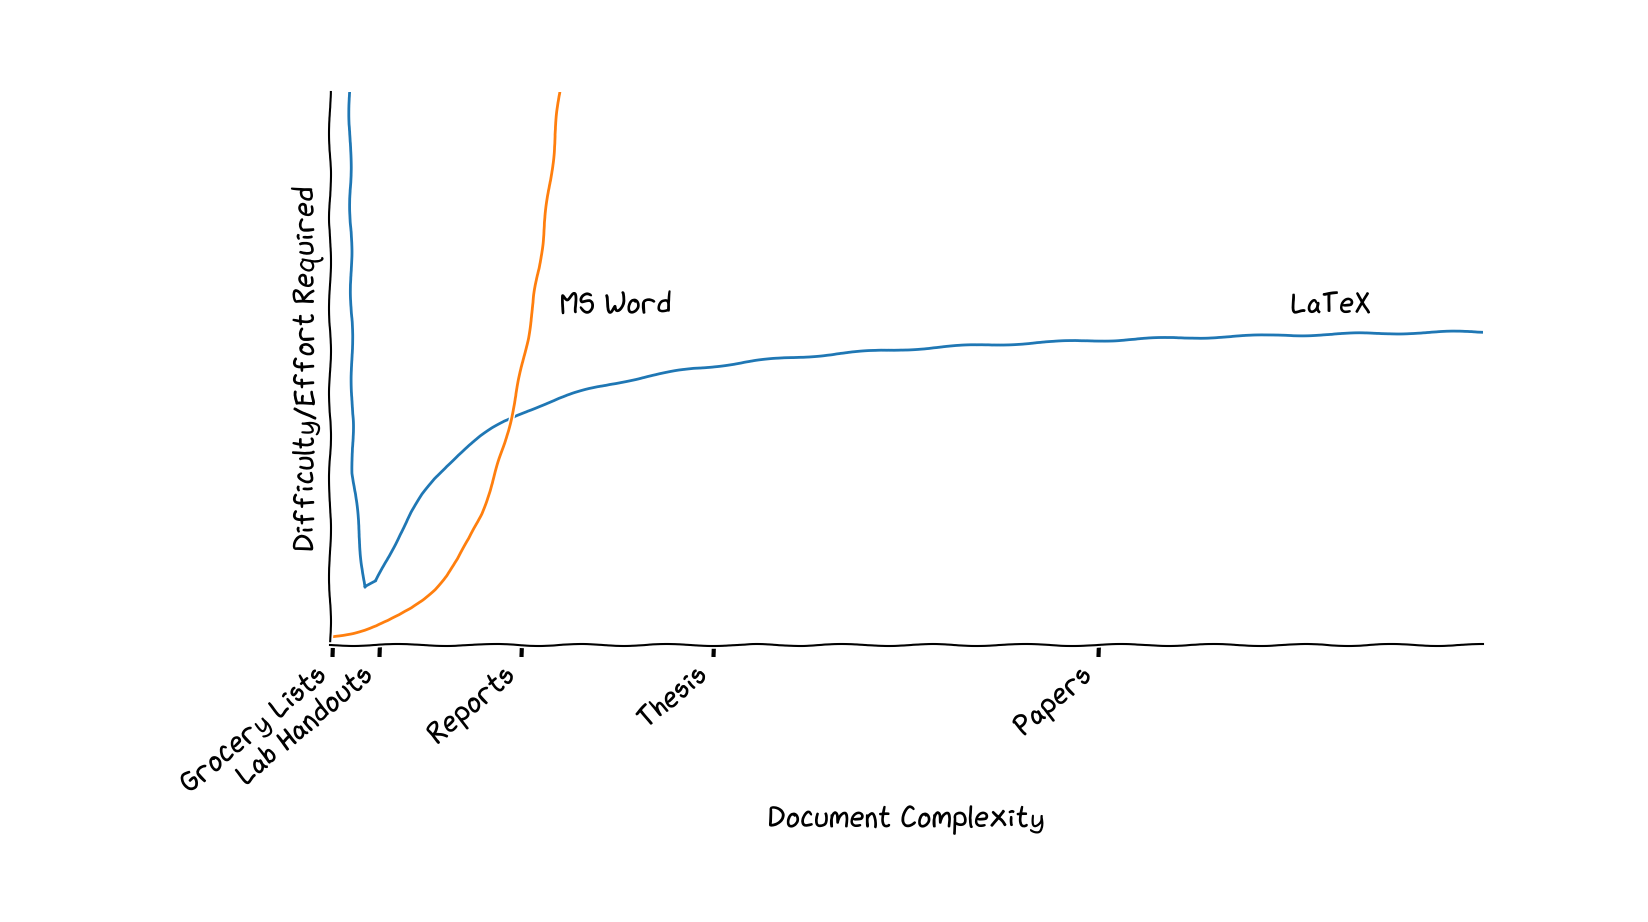
\includegraphics[width=0.75\linewidth]{images/writing_tool_cmp}
	\end{center}
	
	
%	{\let\clearpage\relax \chapter{\LaTeX\ Basics}}
	\chapter{\LaTeX\ Basics}
		
		A \LaTeX\ document consists of the preamble and the main content. The preamble is everything before the \texttt{\textbackslash begin$\lbrace\text{document}\rbrace$} where you import all the packages needed for your document and configure them. Any global definitions also go here.  
		
		
		\section{Document Classes}
		For writing reports we will mostly be using the \texttt{report} document class. There are other alternatives but they are generally not suited for writing reports. If you want to know the differences between the three major classes you can read this \url{https://tex.stackexchange.com/questions/36988/regarding-the-book-report-and-article-document-classes-what-are-the-mai}.
		
		
		\section{Figures and Images}
		Most (good) \LaTeX\ editors will feature an easy way to insert images. TeXstudio for instance has a Insert Graphic Wizard or you can just paste images directly into the editor. Here's an example of how a figure environment is used.
		\begin{figure}[H]
			\begin{subfigure}[h]{0.5\linewidth}
				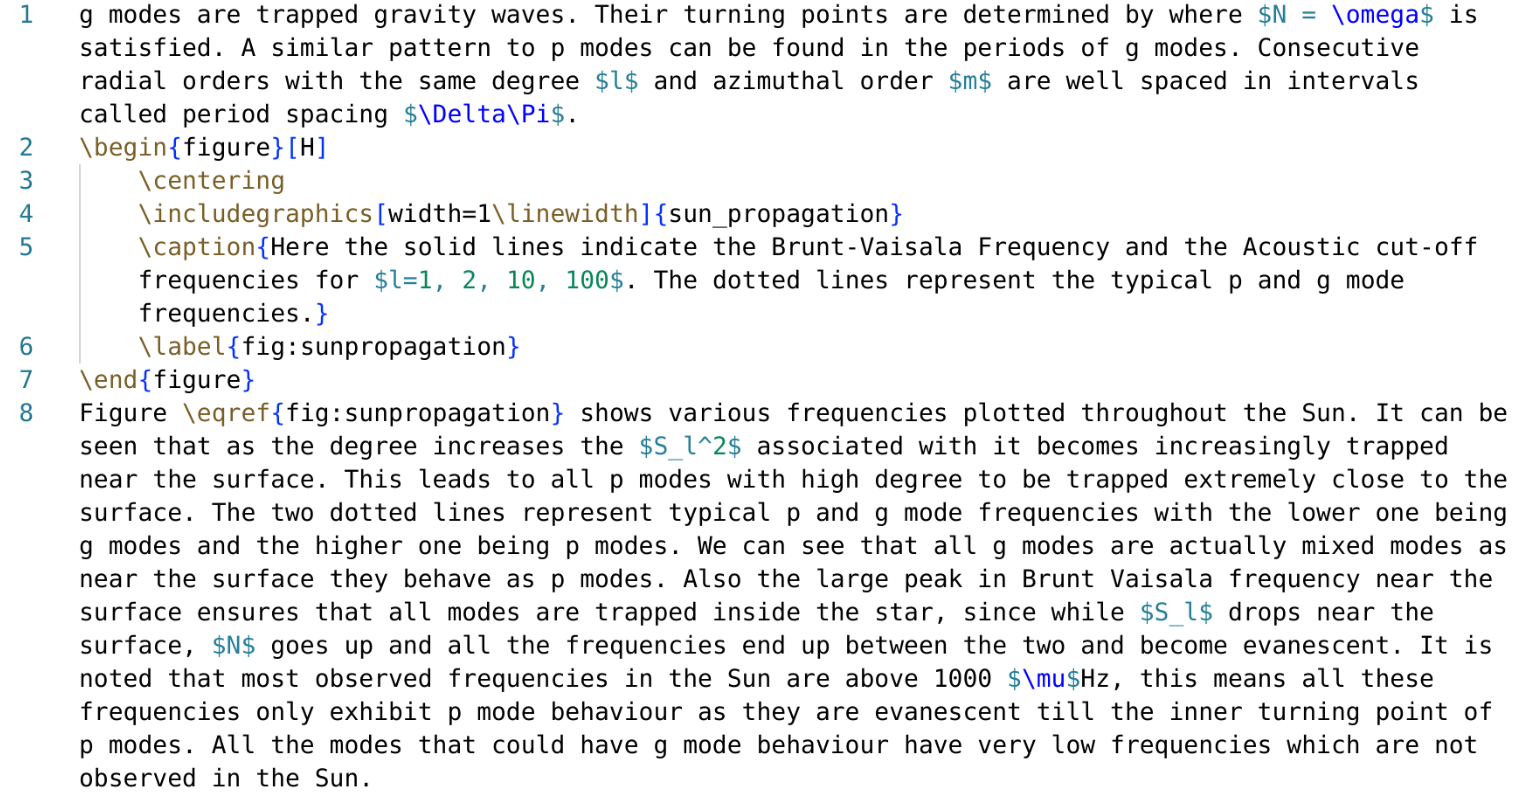
\includegraphics[width=\linewidth]{images/fig_code1.png}
				\caption{The \LaTeX\ code for a figure}
			\end{subfigure}
			\begin{subfigure}[h]{0.5\linewidth}
				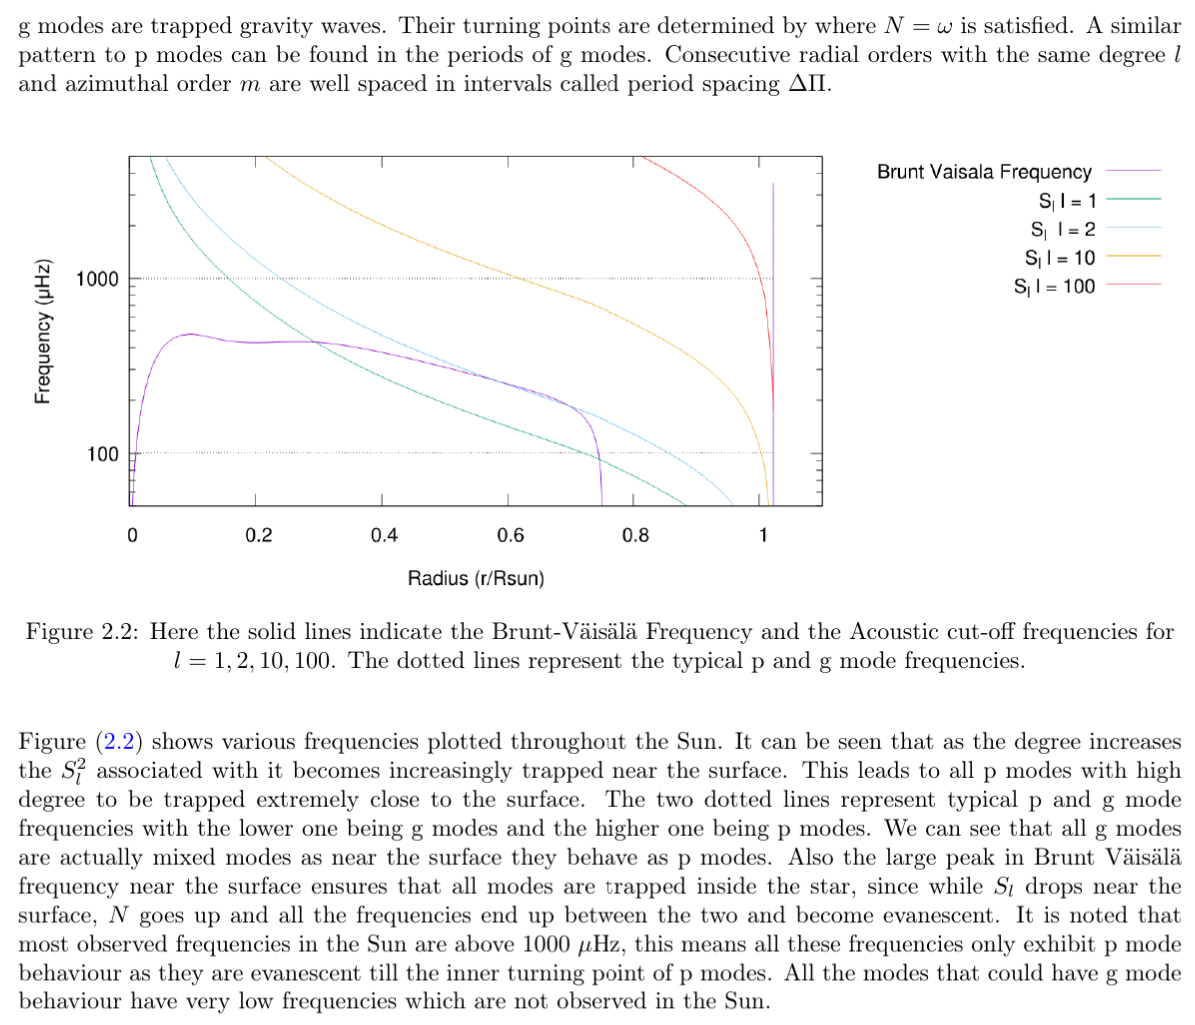
\includegraphics[width=\linewidth]{images/fig_prev1.png}
				\caption{The resulting output}
			\end{subfigure}%
			\caption{An example of a figure environment.\label{fig:fig_example}}
		\end{figure}
		Here the figure environment allows you to position the image by floating it. This means that \LaTeX\ will find a place for it depending on your hints. Personally, we find the \texttt{H} option from the \texttt{float} package to be the best option since it ensures the image stays where it is in the code (as shown in the Figure \ref{fig:fig_example}). Captions are also included in this figure environment and are floated according to the image position.
		
		Generally the image is kept in the same folder but as long as the path is mentioned properly in \lstinline|\includegraphics| it will work fine. When passing the size of the image try not to set both width and height as it will change the aspect ratio of the image. Setting only one of height or width will automatically scale the other to maintain aspect ratio.
		
		A label also helps when you want to refer to the image later. The \texttt{report} class numbers figures and equations based on section and chapter numbers. Figures can also be grouped together into a single figure using subfigures. For example, Figure \ref{fig:fig_example} is a figure with two subfigures. This can be done using \verb*|subcaption| package\footnote{Yea confusing naming.}.
	
		\section{Hyperlinks}
		\begingroup
		If you use the \texttt{hyperref} package a lot of sane basics are applied to hyperlinks. One thing to note is that the default hyperlink style is not particularly great (personal and somewhat subjective opinion), as it renders a box around all your hyperlinks. Changing the default style is quite easy and it can be done in a single line. 
		\endgroup
		\begin{lstlisting}[style=mystyle]
\hypersetup{
	colorlinks = true, % Color links instead of ugly boxes
	linkcolor  = blue, % Color for internal links
	urlcolor   = blue, % Color for external hyperlinks
	citecolor  = red   % Color of citations
	linktoc=all,       % Links in Table of Contents
}\end{lstlisting}
		This snippet sets the hyperlink colors and removes the box around them. \texttt{linktoc=all} makes the sections and subsections linked in the table of contents.
		
	\section{Sections and Chapters}
		A \LaTeX\ report is divided into chapters and sections. This division is important as the default numbering of equations, figures, tables, etc. relies on the current chapter, section and subsection\footnote{and subsubsection but we don't talk about those}. It also helps with maintaining a flow to your report. 
		
		By default each chapter is placed in a new page. This might be what you want for your report but there are times where you would prefer it to be continued in text. This can be done using the following snippet instead of your usual \lstinline[style=mystyle]|\chapter{...}|
		\begin{lstlisting}[style=mystyle]
{\let\clearpage\relax \chapter{...}}\end{lstlisting}
		
		
	\section{Paragraphs}
	There are some things you must be aware of when splitting your content into paragraphs in \LaTeX. All new paragraphs in \LaTeX\ excluding the first paragraph in a section or chapter will have an indent before them. A new paragraph is identified by this indent. It can be seen at many places in this document. A blank line between two blocks of text in your \LaTeX\ source code will create a new paragraph. This is useful as you can separate blocks of code to be more readable without triggering a new paragraph but it also means that you need to be careful with leaving blank lines where you don't intend to start a new paragraph. It should also be noted that \verb*|\\| command does not create a new paragraph, it simply inserts a newline.
	
	{\reversemarginpar\marginnote{\small This is the $\rightarrow$ indent.$\quad$}}You shouldn't start a new paragraph when discussing an equation inside a paragraph. This is easy to do by mistake as leaving a blank line after the equation environment will cause the paragraph to split into two leaving an indent on the text following the equation. 
	
	\section{Equations}\label{sec:equations}
	Typesetting equations is one of the biggest advantages of using \LaTeX\ and one of the the biggest reasons why the effort required to write more academically complex documents goes up very slowly when using \LaTeX\ (Refer to Figure on page 1). \LaTeX\ features a math mode which allows you to write equations in a symbolic form. This way of writing equations has become ubiquitous in most methods of typesetting and is the most stereotypical form of ``\LaTeX''.
	
	Math mode can be used either inline by enclosing commands in \verb*|$...$| (which produces something like this $e^x$). Inline mode doesn't give you equation numbers and doesn't put the math on a separate line. The other method involves using the \texttt{equation}, \texttt{align}, \texttt{gather}, ... environments. These environments put the equations on a separate line and add equation numbers. For example
	\begin{equation}
		F = ma.
	\end{equation}
	
	With parenthesis of any kind try to use \lstinline|\left| and \lstinline|\right|. They allow you to automatically balance brackets and more importantly they resize automatically based on its contents. This makes a significant difference in larger equations and makes them way more readable. Here's an example,
	\begin{gather}
		\bm{\times} \qquad\qquad\qquad\qquad\qquad \checkmark \nonumber\\
		[a^2 + (e^{\int_0^{\infty} f(t) \text{d}t})b^2] ,\qquad\qquad  \left[a^2 + \left(e^{\int_0^{\infty} f\left(t\right) \text{d}t}\right)b^2\right].
	\end{gather}
	
	Over time you'll find that you keep using some snippets over and over again. This would be a good time to write a few of your own macros/commands. This will save you a lot of time. \LaTeX\ allows you to define your own commands and even redefine existing ones. For example a command for derivatives can be defined as follows
	\begin{lstlisting}[style=mystyle]
\newcommand{\deriv}[3][]{\frac{d^{#1} #2}{d #3^{#1}}}\end{lstlisting}
	Commands can also be redefined for example, \lstinline[style=mystyle]|\div| command can be defined to be divergence instead of the division symbol as follows
	\begin{lstlisting}[style=mystyle]
\renewcommand{\div}{\,\textnormal{div}\,}\end{lstlisting}

	Sometimes, willingly or otherwise, you will be left with an equation too large for a single line. In these situations you can use the \verb*|align|, \verb*|gather| or \verb*|multiline| environments. The exact syntax can be found online but one should use \verb*|align| when you need to write multiple steps and you want them to be aligned to the equals to sign, for example,
	\begin{align}
		Z[J] &\equiv \int{D\Phi \, \text{exp}\left[i \int{d^4 x}(\mathscr{L}[\Phi]+J\Phi)\right]} \nonumber \\
		&= \text{exp}\left(i \int{d^4x}\mathscr{L}_1\left[i \frac{\delta}{\delta J}\right]\right) \text{exp}\left(i \int{d^4x }(\mathscr{L}_0 +J\Phi) \right) .\label{eq:Z}
	\end{align}
	
	You should use \verb*|gather| when you just need the multiple lines of the equation to just be center aligned, for example,
	\begin{gather}
		\delta g^{\mu\nu} = - g^{\mu \rho}g^{\nu \sigma} \delta g_{\rho \sigma}, \\
		\delta g_{\mu\nu} = - g_{\mu \rho}g_{\nu \sigma} \delta g^{\rho \sigma}, \\
		\delta g  = g g^{\mu\nu} \delta_{\mu\nu}, \\
		\delta \sqrt{-g}  = \frac{1}{2}\sqrt{-g} g^{\mu\nu} \delta_{\mu\nu}. \label{eq:var-detg}
	\end{gather}
	
	The last one is \verb*|multiline| which you use when you don't have a particular use case but you still need multiple lines, for example if the equation is way too large for a single line like so	
	\begin{multline}
		\rho(\eta,\mathbf{x})=\expv{\varrho(\eta,\mathbf{x})} \nonumber \\
		= \rho_0(\eta)+a^{-4}\frac{3\lambda}{4!}  \left( \int_{\mathbf{k}} |\chi_k(\eta)|^2\right)^2 +a^{-4}\frac{12\lambda}{4! } \operatorname{Im}
		\left\{ \int_{-\infty}^{\eta}{d\tau} a^4(\tau) \left\{  \int_{\mathbf{k}}\left[ \chi'_k(\eta) \chi^*_k(\tau) \right]^2 \right. \right. \nonumber \\
		\left. \left.+\int_{\mathbf{k}} \left[ \omega_k^2(\eta)+(1-6\xi)\mathcal{H}^2(\eta)\right] [\chi_k(\eta) \chi_k^*(\tau)]^2 +(1-6\xi)\mathcal{H}(\eta) \int_{\mathbf{k}}\chi_k(\eta)\chi'_k(\eta)  [\chi_k^*(\tau)]^2 \right\} \left[\int_\mathbf{k}|\chi_k(\tau)|^2\right] \right\}.\label{eq:interacting energy density}
	\end{multline}
	
	
	
	In the last example \lstinline|\left| and \lstinline|\right| will not be balanced since they are on different lines. They can be made to balance by using a \lstinline|\right.| to virtually close the bracket. You can read the source code of this document to see how the equation is written or you can read about other ways of doing this \href{https://tex.stackexchange.com/questions/21290/how-to-make-left-right-pairs-of-delimiter-work-over-multiple-lines}{here}.

\section{Bibliography}
Bibliography is yet another reason \LaTeX\ is incredible for academic contexts. While some word processors do provide ways to manage bibliographies and citations, they all reimplement the same citation system that \LaTeX\ uses. There are many packages that provide bibliographies in \LaTeX. We recommend you read \url{https://www.overleaf.com/learn/latex/Bibliography_management_in_LaTeX} for a proper tutorial/guide to bibliography in \LaTeX. They do a much better job than we could in this small document.

Our advice for bibliography would be to copy over references of all papers you read into your \texttt{bib} file. While you might not end up citing all of them it is easier to find them if you keep a record from the beginning. 

\newpage
\section{Some specific tips and tricks}
\begin{itemize}
	\item \textbf{Code Snippets}
	\begin{itemize}
		\item Use the \texttt{lstlistings} package. However, you might have to define a style to make the code blocks look decent since the default is quite barebones.
		\item If you include julia code especially those containing unicode characters such as greek letters you may want to use \url{https://github.com/wg030/jlcode}
	\end{itemize}
	\item There exists a \texttt{physics} package that provides macros and styles for many of the commonly used objects in physics. However, we personally didn't like the package since we already had macros that did the same things in our own taste.
	\item Setup your hyperlinks properly as it makes a document much easier to navigate. Ensure that the table of contents is properly linked. Citation, equation and figure links are quite important as well since it allows the reader to jump to what you are talking about. 
	\item You can use \lstinline|\includepdf| from the package \verb*|pdfpages| to include things like certificates. Once you get the signed certificate as a pdf file you can always just include it in your document as a page making this process quite easy and seamless.
	\item Modify \verb|\vec| to use boldface instead of a overdrawn arrow. This is the standard in nearly all physics literature. ($\vec{a}$ vs $\bm{a}$). This can be done with the following snippet included somewhere in your preamble.
	\begin{lstlisting}[style=mystyle]
\renewcommand{\vec}[1]{{\bm{#1}}}\end{lstlisting}
	\item \textbf{Astrophysics}
	\begin{itemize}
		\item ADS references are designed for papers that use a custom \LaTeX\ style provided by journals. You will get many errors if you try to use references generated from ADS as the journal names are defined by \LaTeX\ commands such as \verb*|\apj|, \verb*|\aap|, etc. You can extract just the journal definitions from the AAS style classfiles \footnote{They can be found here \url{https://journals.aas.org/aastex-package-for-manuscript-preparation/#_download}. You can open any classfile and search for lines starting with \verb*|\newcommand| containing \verb*|\aap| or similar journals to find the definitions.}. If this proves difficult you can drop us a mail and we'll can share a file with the definitions.
		\item Define a few helper commands for solar mass and other units. There is probably a package for this but this is pretty easy to do by hand.
	\end{itemize}
	\item \textbf{Particle Physics and Quantum Field Theory}
	\begin{itemize}
		\item Use the \texttt{tikz-feynman} package to draw Feynman Diagrams. A good documentation can be found \href{https://in.mirrors.cicku.me/ctan/graphics/pgf/contrib/tikz-feynman/tikz-feynman.pdf}{here.}
		\item Wick contractions can be done using the package \verb*|simpler-wick|.
	\end{itemize}
\end{itemize}	

	\chapter{Report Writing}
	\begin{tcolorbox}[colback=red!5!white,colframe=darkred!75!black,title={\large \textbf{An Advisory on ChatGPT and other LLMs}}]
		While LLMs such as ChatGPT are a technological marvel and are incredibly useful tools, they must be used with extreme caution in a academic setting. The usage of LLMs for writing \LaTeX\ code is relatively harmless as long as your check for errors and ensure your content is unmodified. However, LLMs must \textbf{never} be used for writing your report for you, coming to conclusions using your data or sifting through data. \bigskip
		
		While it is also a question of academic integrity there is a more pressing problem with using LLMs for this purpose. LLMs are all biased to their training data. Using an LLM for research risks tainting your entire work with that bias. For fields such as ours where we must strive to be as objective as possible, a system that is inherently biased should be used judiciously and with caution.
	\end{tcolorbox}
	\section{General Advice}
	\begin{itemize}
		\item \textbf{Never write anything you don't know.} A report is a compilation of your work and knowledge. 
		\item \textbf{Cite everything you didn't explicitly do yourself.} This includes figures, data, results, derivations, etc.
		\item \textbf{Define every symbol.} Never assume a symbol has standard meaning. 
		\item \textbf{Maintain a bibliography.} BibTeX makes this extremely simple. Most websites that host scientific literature have an export citation feature. Copy the BibTeX code into a references file for every paper that you read. Never leave citations till the end of a report. 
		\item \textbf{Give ample background.} Reports are not papers, they will be read in isolation. You cannot assume more than proficiency in science.
		\item \textbf{Maintain a flow.} Start your sections with a brief explanation of their contents to motivate the readers. This is common practice in many papers and helps make your report more readable. You should also make sure that you never need information from later sections to understand an earlier section. For example, a derivation in Section 2 should not require information from Section 3.
		\item \textbf{Typeset your equations well.} Refer to Section \ref{sec:equations} for tips to do this. Equations are often the essence and hardest parts of reports. They need to be perfect for your report to look good.
		\item \textbf{Get a friend,} or two. You need someone to correct your typos, misaligned paragraphs, mismatched brackets and other mishaps which are entirely invisible to the author themselves.
		\item \textbf{Collect often used snippets of code.} As your write reports you will notice that you write certain bits of text a lot. Collect these together and reuse them as they will save you a lot of time and will help make your \LaTeX\ code more readable in the long run.
		\item \textbf{Punctuate equations.}
		While equations can appear on their own they are still technically part of the sentence. You must add punctuation after the equation depending on whether you plan on continuing the sentence. For instance, if you take an equation such as
		\begin{equation}
			\bm{\delta r} = \sqrt{4\pi} Re\left\lbrace\left[\tilde{\xi}_r\left(r\right) Y^m_l\left(\theta, \phi\right) \bm{a}_r + \tilde{\xi}_h\left(r\right) \left(\partialderiv{Y^m_l}{\theta} \bm{a}_\theta + \frac{1}{\sin \theta} \partialderiv{Y^m_l}{\phi} \bm{a}_\phi\right)\right] \exp \left(-i\omega t\right)\right\rbrace,
		\end{equation}
		{\reversemarginpar\marginnote{\uprightarrow \\\small Notice how the paragraph is continued after the equation. There is no indent here and no new paragraph.}[1.2mm]}in the middle of a sentence you'll need to use a comma instead of a full stop. This works wonders in making your report look more professional and the difference is immediately obvious even though it feels like a minute detail.
		\item \textbf{Get feedback,} submit your report ahead of time even if it is just a draft to your guide or project instructor for advice. They can help you a lot more than you expect and won't be crunched for time.
	\end{itemize}
	
	\appendix
	
	\chapter{Final Checklist}
	\large
	\begin{todolist}
		\item Get your certificates signed, \textbf{ahead of time}.
		\item Check that everything is cited.
		\item Check equations for punctuation.
		\item $\square$ $\square$ Check typos and grammar, at least thrice.
		\item Ensure all figures have labelled axes.
		\item Ensure your floats (tables and figures) are in the right place.
		\item Make sure your original work is highlighted. The work of others should be cited or acknowledged and at most discussed.
		\item Acknowledge everyone who can't be cited.
		\item Don't plagiarise and don't worry about plagiarism checkers if you didn't\\ plagiarise.
	\end{todolist}
	
\end{document}